\chapter{Introduction}
\label{chap:introduction}
%%%%%%%%%%%%%%%%%%%%%%%%%%%%%%%%%%%%%%%%%%%%%%%%%%%%%%%%%%%%%%%
% OUTLINE FOR INTRODUCTION 
% 1. Quick introduction of topic
    % 1.1. Traditional methods of identifying probelmatic data
    % 1.2. Machine Learning applied to more and more mundane tasks
% 2. Problem statement
    % 2.1. What is the problem?
    % 2.2. Why is it important?
% 3. Scope
    % 3.1. What is the current landscape? 
    % 3.2. How does this fit into that landscape
% 4. Objectives
    % 3.1. What does this add to the current landscape?
% 5. Structure of the thesis
    % 5.1. What is the structure of the thesis?
%%%%%%%%%%%%%%%%%%%%%%%%%%%%%%%%%%%%%%%%%%%%%%%%%%%%%%%%%%%%%%%

%% Segev Outline for Introduction
% 
% SN classification & Identification: Why important?
% Spectra as "gold standard" for classifiers 
% Attempt at spectroscopic classification
% Madgwich et al, Gravr et al (2013), Bovan et al, Mathukrishna et al (2019)
% AI/ ML approach: why better, possibly? 
% What problems does it solve
% what will you be looking at 
% i.e. de-redshifted vs not, subtypeclassification vs none, etc.
% "We will explore the following questions:

% SYB Comments:
% - There is a long history of naked-eye observations of supernovae that predates the invention of the telescope. The most well-known is probably SN 1054, which we now observe as the Crab Nebula.
% - Despite millennia of observations, the nature of these explosions was not really understood until the 1930s. It might be interesting to discuss why.
% - You don't explain what supernovae are: the end stage of the life-cycle of a massive star (usually $$>8 M_\odot$). More rarely (about 1/3 of the time) they are explosions in binary systems involving one WD star + a massive companion sharing a stellar envelope.
% - You can work these facts in, with sufficient citations.

When observing the night sky, astronomers frequently encounter objects that 
are unexpected. This occurred quite frequently in the 19th century, as astronomers 
armed with more powerful telescopes were probing the cosmos for the first time. 
In 1885 and 1895, two objects were observed in galaxies outside of our own with unique 
properties \parencite{deVaucouleurs1985, Schaefer1995}. These objects were very 
bright, outshining their host galaxies, and faded away over the course of a few months.
These objects were eventually named `supernovae' (SNe) by Walter Baade and Fritz Zwicky, who were the first to suggest that
these objects were the result of the death of a star, and predict the resulting 
object to be a cold, neutron star\parencite{Baade1934}. Since then, astronomers 
have observed thousands of SNe~\parencite{Barbon1999}, and have
developed a classification scheme for these objects.  

\section{Supernova Classification}
\label{sec:supernova-classification}
SNe have been traditionally classified based on their spectra starting with 
\textcite{Minkowski1941}, who first classified SNe into two groups based on the
presence or absence of hydrogen lines in their spectra. This classification provided 
the basis for the current classification scheme, which is based on the presence
or absence of hydrogen and silicon in the spectra of SNe. This classification 
scheme is shown in Figure~\ref{fig:sn-classification}. 

\begin{figure}[ht]
    \centering
    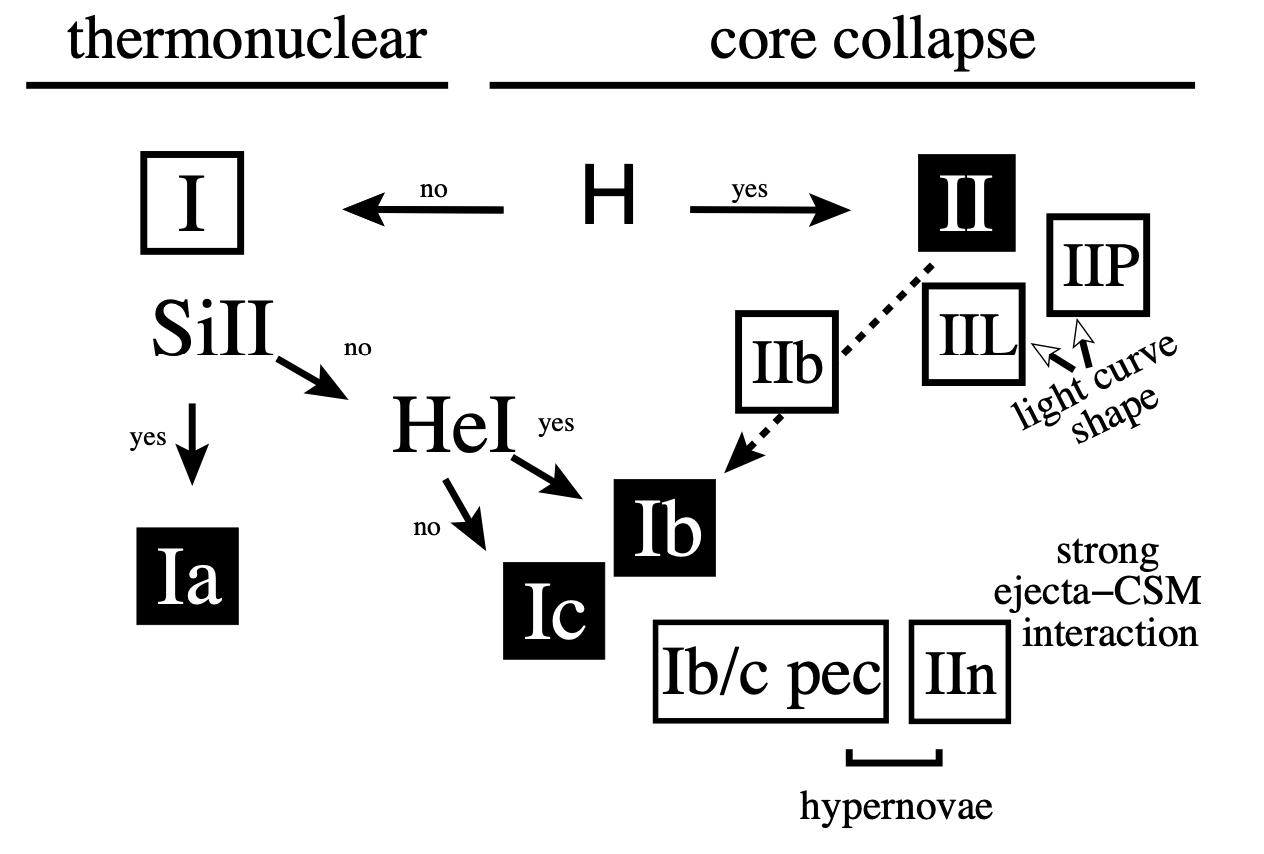
\includegraphics[width=0.8\linewidth]{figures/supernova_class.png }
    \caption[Supernova Classification]{Supernova classification. The 
    classification scheme is based on the presence or absence of hydrogen and 
    silicon features in the spectra of SNe. Figure from \textcite{Turatto2003}.}
    \label{fig:sn-classification}
\end{figure}

% The classification scheme in Figure~\ref{fig:sn-classification} is based on
% the presence or absence of hydrogen and silicon emission and absorption lines in the spectra of SNe.
SNe with hydrogen in their spectra are classified as Type II SNe, while those
without hydrogen are classified as Type I SNe. Type I SNe are further
subdivided into Type Ia, Ib, and Ic~\parencite{Turatto2003}. Although divided into three 
subtypes, Type I SNe are caused by two different mechanisms. Type Ia SNe are 
caused by the thermonuclear explosion of a white dwarf star, while Type Ib and Ic 
SNe are caused by the core-collapse of a massive star~\parencite{Filippenko1997}.
Type Ib and Ic SNe, because of this, are actually more related to Type II SNe,
and are collectively referred to as core-collapse SNe. We now know the physical
origin of the spectral differences between the subtypes: stars stripped of their 
hydrogen envelopes are appear as Type Ib SNe, while those stripped of both their 
hydrogen and helium envelopes are classified as Type Ic SNe.

\section{Supernova Identification}
\label{sec:supernova-identification}
The different types of SNe are caused by different mechanisms, and therefore 
knowing the type of a SN can provide insight into the mechanism that caused it.
Merely detecting a supernova is therefore not enough; astronomers must also identify its
type to identify its origin. Traditionally, a supernova is observed by several 
means, with discovery in photometric observations and classification using follow-up spectroscopy (e.g. \textcite{Perlmutter1999}). This process is time-consuming, requiring not only 
the initial discovery of the supernova, but also follow-up observations to determine
the type before it fades away. Today, due to the large volume of new discoveries and the small number of single and multi-object spectrographs suitable for follow-up, only about 10\% of discovered SNe receive spectroscopic classification.
% Citation on this could be the Transient Name Server.

\section{Dark Energy Spectroscopic Instrument}
\label{sec: DESI}
* Write a section about DESI
* What is it?
* Why is it important?
* Why do we care about SNe here

See the intro and instrument sections of this paper: https://arxiv.org/pdf/2209.14482.pdf.
You don't need to copy everything. I think 2 paragraphs should be sufficient for this section.
One thing you want to emphasize is the Bright Galaxy Survey, which is where most of these transients
are being observed. A question you should be able to answer: at what redshifts are we looking for 
these transients? (Basically anything with $z<0.25$.

% https://docs.google.com/presentation/d/14i0USbCQ93Mkn1T9aUK5pG24bi5bRfBhM3aVsL1Ya0U/edit?usp=sharing
% -- Look at spectra examples
% -- Look at motivation for no-redshift corrected transient classification

% https://docs.google.com/presentation/d/1zqoEVMrWbBP5k41gdjUEKioLE4J0vhu0vAzKEg4pROM/edit?usp=sharing
% -- An old presentation from 2020 that lists some past approaches to spectroscopic classification.
% -- Supernova tempates and compared them 
%   - Fit forgrown spectra from galaxy, fit residual spectrum. CHi^2 fit looks good?you discover it
% -- Type 1A evolution
%   - You can't just compare to one, you need to compare to A BUNCH because of time 
%   - So you want to compare to every template?? Convolve at different redshifts??
%   - SUUUPER expensive. ML/AI is just... better. 


\section{Supernova Classification with Machine Learning}
\label{sec:supernova-classification-with-machine-learning}

% SB Comments:
% You want to motivate this in a couple of ways.
% 1) Because spectroscopic follow-up is tough, it's worthwhile to try to discover SNe serendipitously in spectra rather than only wait for discoveries in imaging surveys.
% 2) The issue with spectroscopic discovery is that you have potentially thousands of templates to compare against (all the different subtypes * all the variants of the subtypes * the spectral evolution of each variant * convolution vs redshift). Very computationally expensive!

I suggest you give some background on previous approaches before jumping right into AI/ML.
See the early slides in \href{https://docs.google.com/presentation/d/1zqoEVMrWbBP5k41gdjUEKioLE4J0vhu0vAzKEg4pROM/edit?usp=sharing}{this Google slideshow}.

Machine learning (ML) has been applied to many different fields for its flexibility 
and ability to find patterns in data. The emergence of Deep Learning (DL) has
allowed ML to be applied to more and more mundane tasks, such as image
classification~\parencite{krizhevsky2012}, speech recognition~\parencite{Nassif2019},
and natural language processing~\parencite{Mikolov2013}. ML and DL 
has also been applied to astronomy, with some success. \textcite{Gauci2010} used 
a random forest algorithm  to distinguish between spiral, elliptical, and irregular galaxies, 
and \textcite{Becker2021} used a convolutional neural network (CNN) to classify the morphology of
radio galaxies. CNNs found success in working within the DESI collaboration, with 
\textcite{parks2018} using the architecture to detect strong emission lines.  
These techniques have also been applied to the classification of SNe. 
\textcite{Mller2016} used a CNN to classify SNe into Type Ia and non-Type Ia SNe. 

\section{Problem Statement}
This work will explore the following questions: how can we adapt novel deep learning 
techniques to classify SNe in the DESI dataset? Can we use this architecture to 
classify SNe into their respective subtypes accurately? And how can we decrease the amount of 
pre-processing required to classify these SNe accurately? In the following chapters,
we describe the Deep Learning techniques adopted to answer this problem (Ch. 2);
the training procedure for building our classification network (Ch. 3);
and the results using simulated DESI spectra that were resampled from actual 
DESI measurements performed in 2021 and 2022 (Ch. 4).

